% \section{Part III: Nonlinear Dimensionality Reduction (for dataset B)}

% Dataset B was partitioned to contain only the digit "3" for parts 1 and 2 of this section. Figure~\ref{fig:fig8} displays all the hand written digits "3" available in the subset. Looking at the images qualitatively, not all "3's" are drawn equally. Images differ with respect to: tilt (either left or right), line weights (thick or thin), width and curvature, to name a few features. 
% \begin{figure}[htb]
%  \centering
% 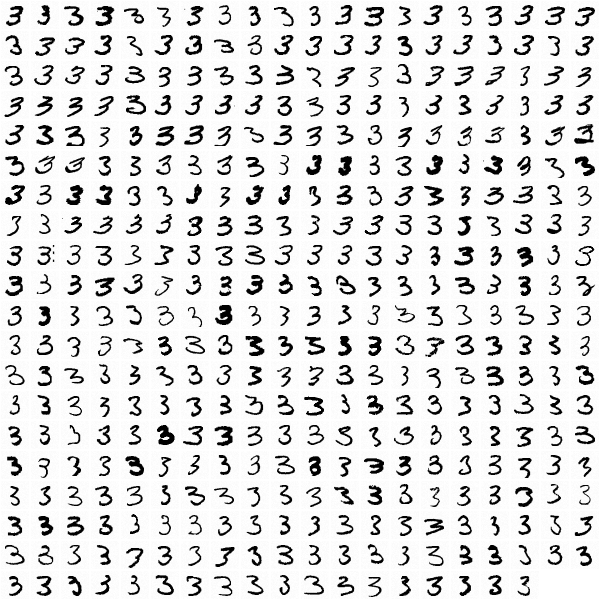
\includegraphics[width=4in]{assignment1/3-0-alldigit3.png}
% \caption{\label{fig:fig8}This gives us an idea of the variety of handwriting styles for digit 3 in the dataset}
% \end{figure}


% \clearpage{}
% \subsection{Apply LLE to the images of digit '3' only}
% The LLE mapping was applied to reduce the number of dimensions to 2. The original images were plotted against the LLE coordinates and can be see in Figure~\ref{fig:fig9}. We can see that the digits on the left side towards the center are tilted right, while the digits on the right side are straight with the exception of a few at the top right corner tilted left. And keeping in accordance to the direction of the digits, the digits on the lower right part  have thinner strokes, while the digits at the left and  near the left part have thicker strokes. Majority of the weird '3's tend to be near the right center to the lower right  corner. There is a very clear pattern of where the images are placed. LLE did the best in mapping the digits in the reduced dimensions. 


 
% \begin{figure}[htb]
%  \centering
% 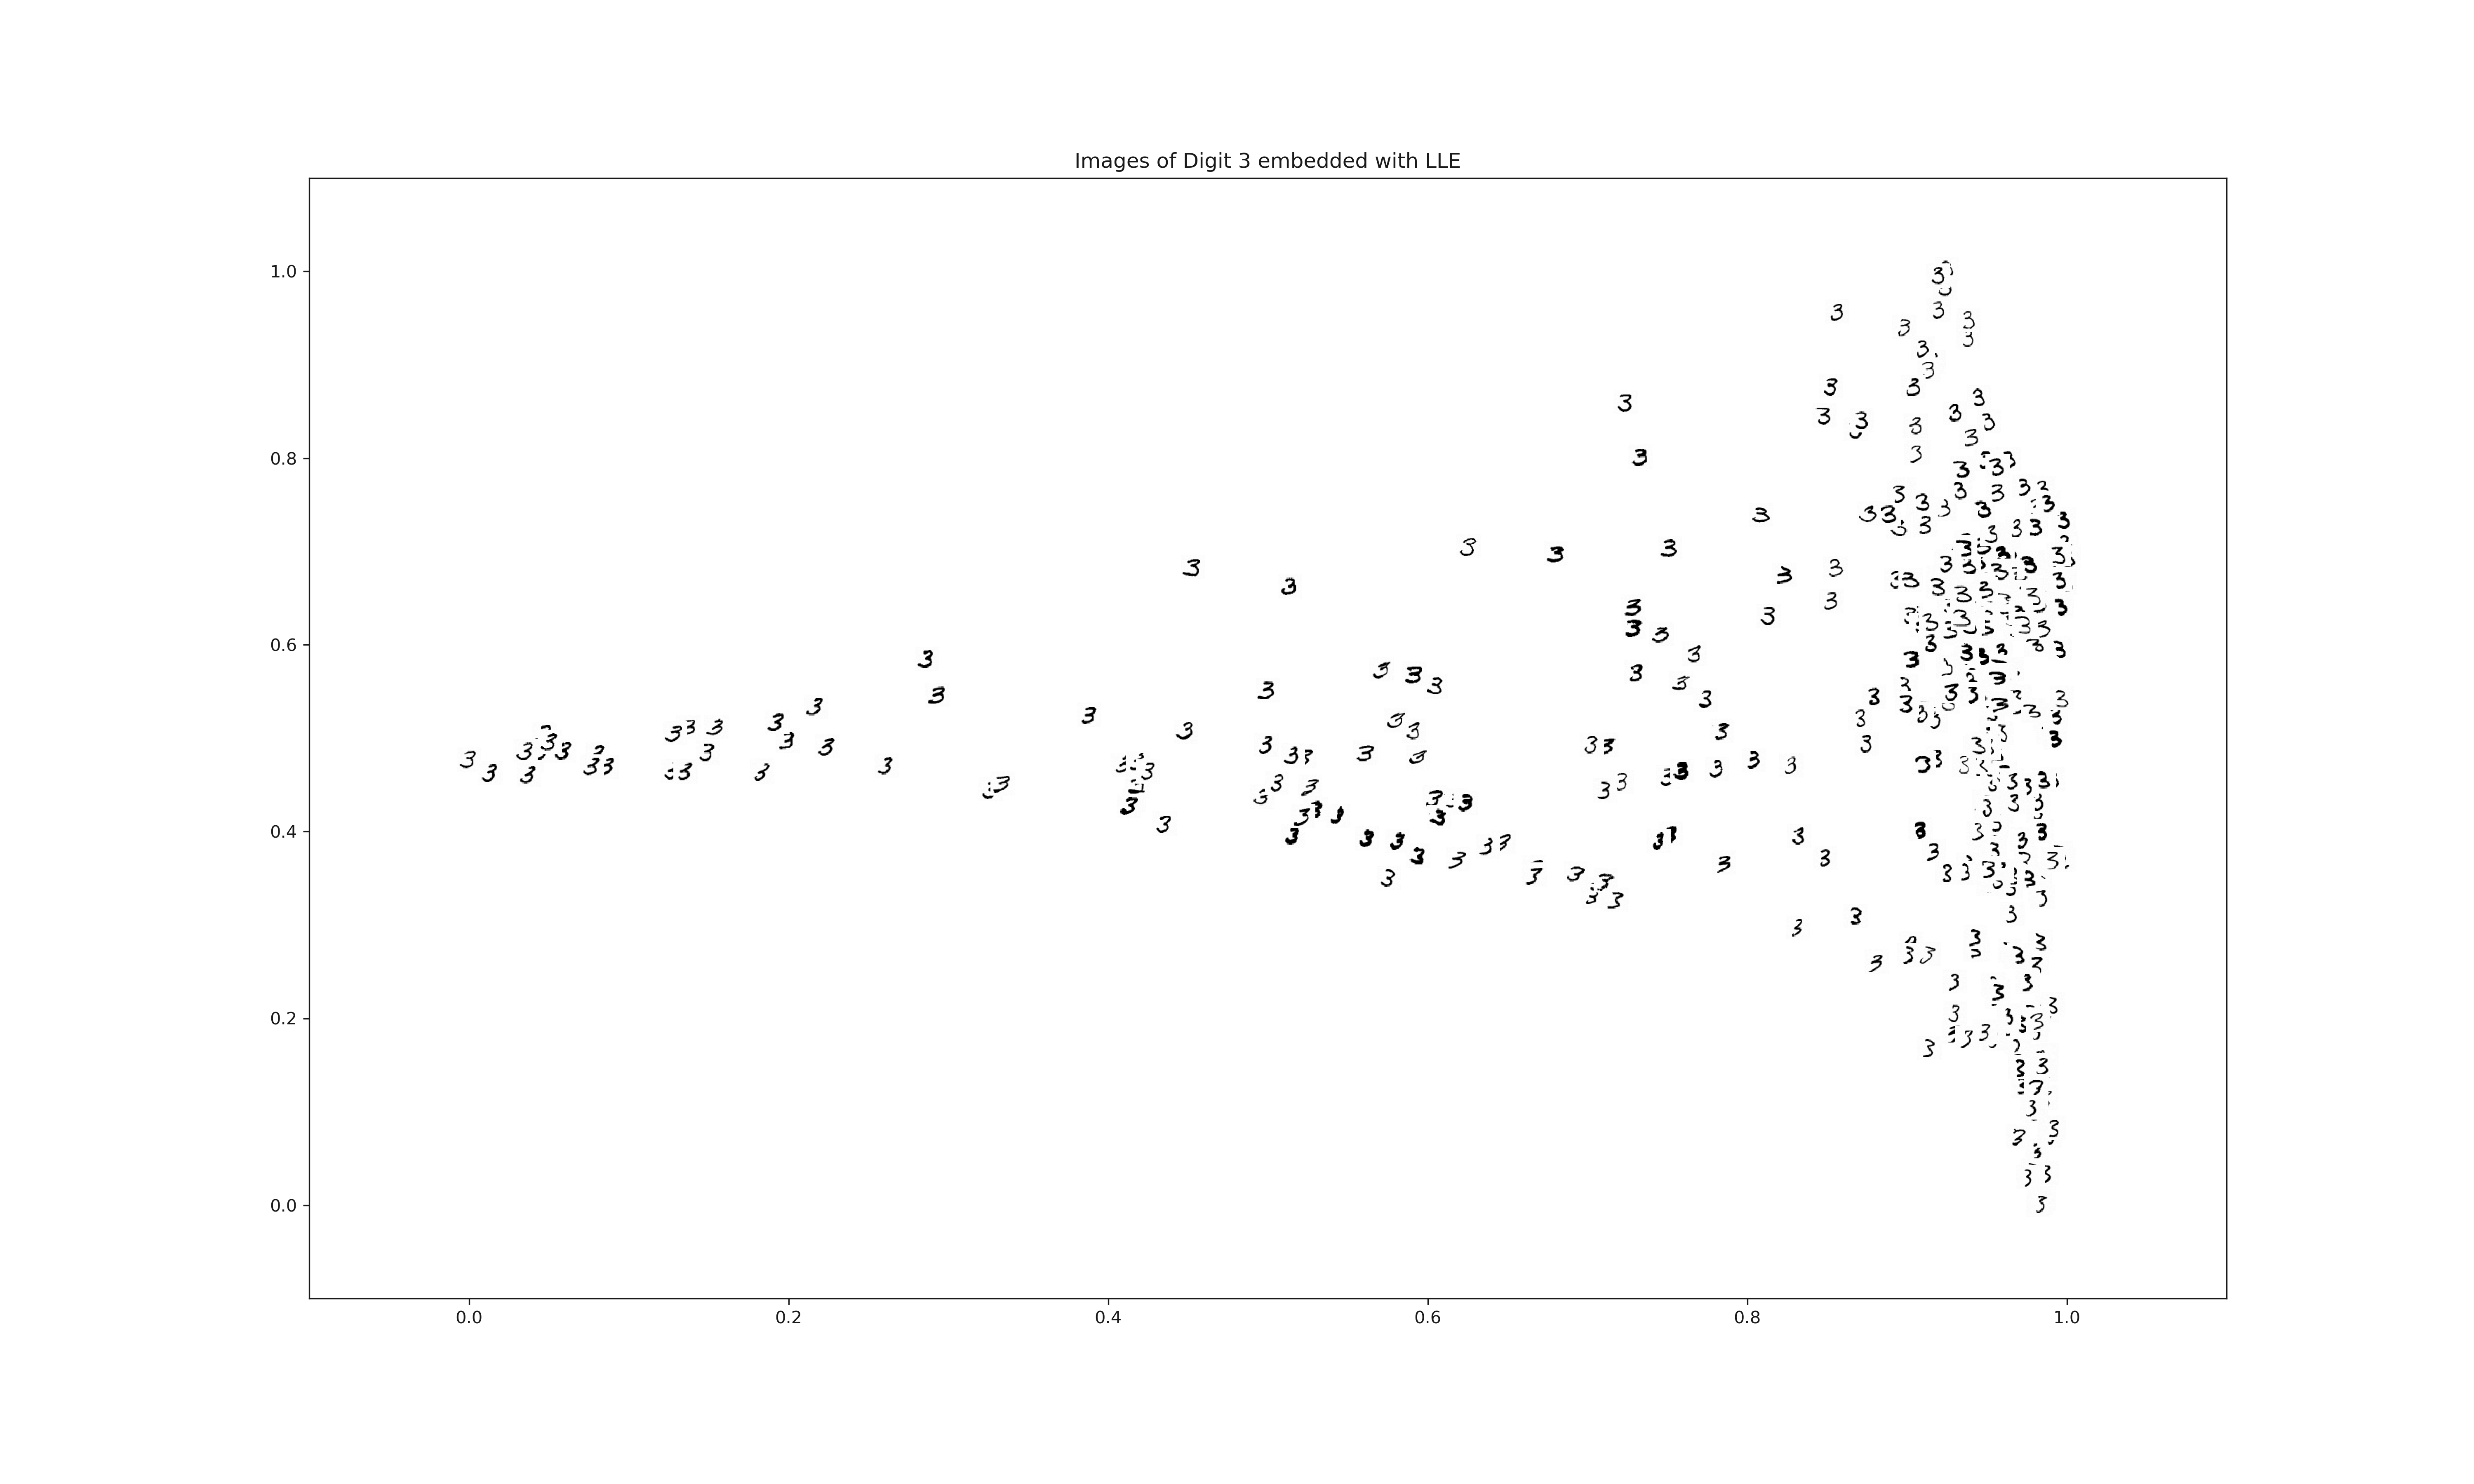
\includegraphics[width=\textwidth]{assignment1/3-1-LLEembedding.png}
% \caption{\label{fig:fig9}Images of digit "3" embedded with LLE}
% \end{figure}



% \clearpage{}
% \subsection{Applying ISOMAP to the images of digit '3' only}

% ISOMAP was used to embed the original images of digit "3" and can be seen in Figure~\ref{fig:fig10}. The result gives an idea of the variety of forms that the digit "3" can take within the dataset. The data lies from left to right in the projected space, which appears to trace the orientation of the digit.We can see that going from left to right of the graph, the digits generally go from tilted to the right to tilted to the left, as you move towards the middle and top center of the plot, you find three's that are partially written or look like other digits and some digits with weak strokes. Isomap did quite better in mapping the digits both by direction and by thickness. Isomap dimensions seem to describe global patterns of the digits: the overall tilt to the right or tilt to the left of the digit from left to right. Overall ISOMAP does not do as well as LLE in grouping the digits with similar features in distinguishable groupings. The digits are much more spread out and this could cause prediction issues if the other digits are included in the mapping.

% \begin{figure}[htb]
%  \centering
% 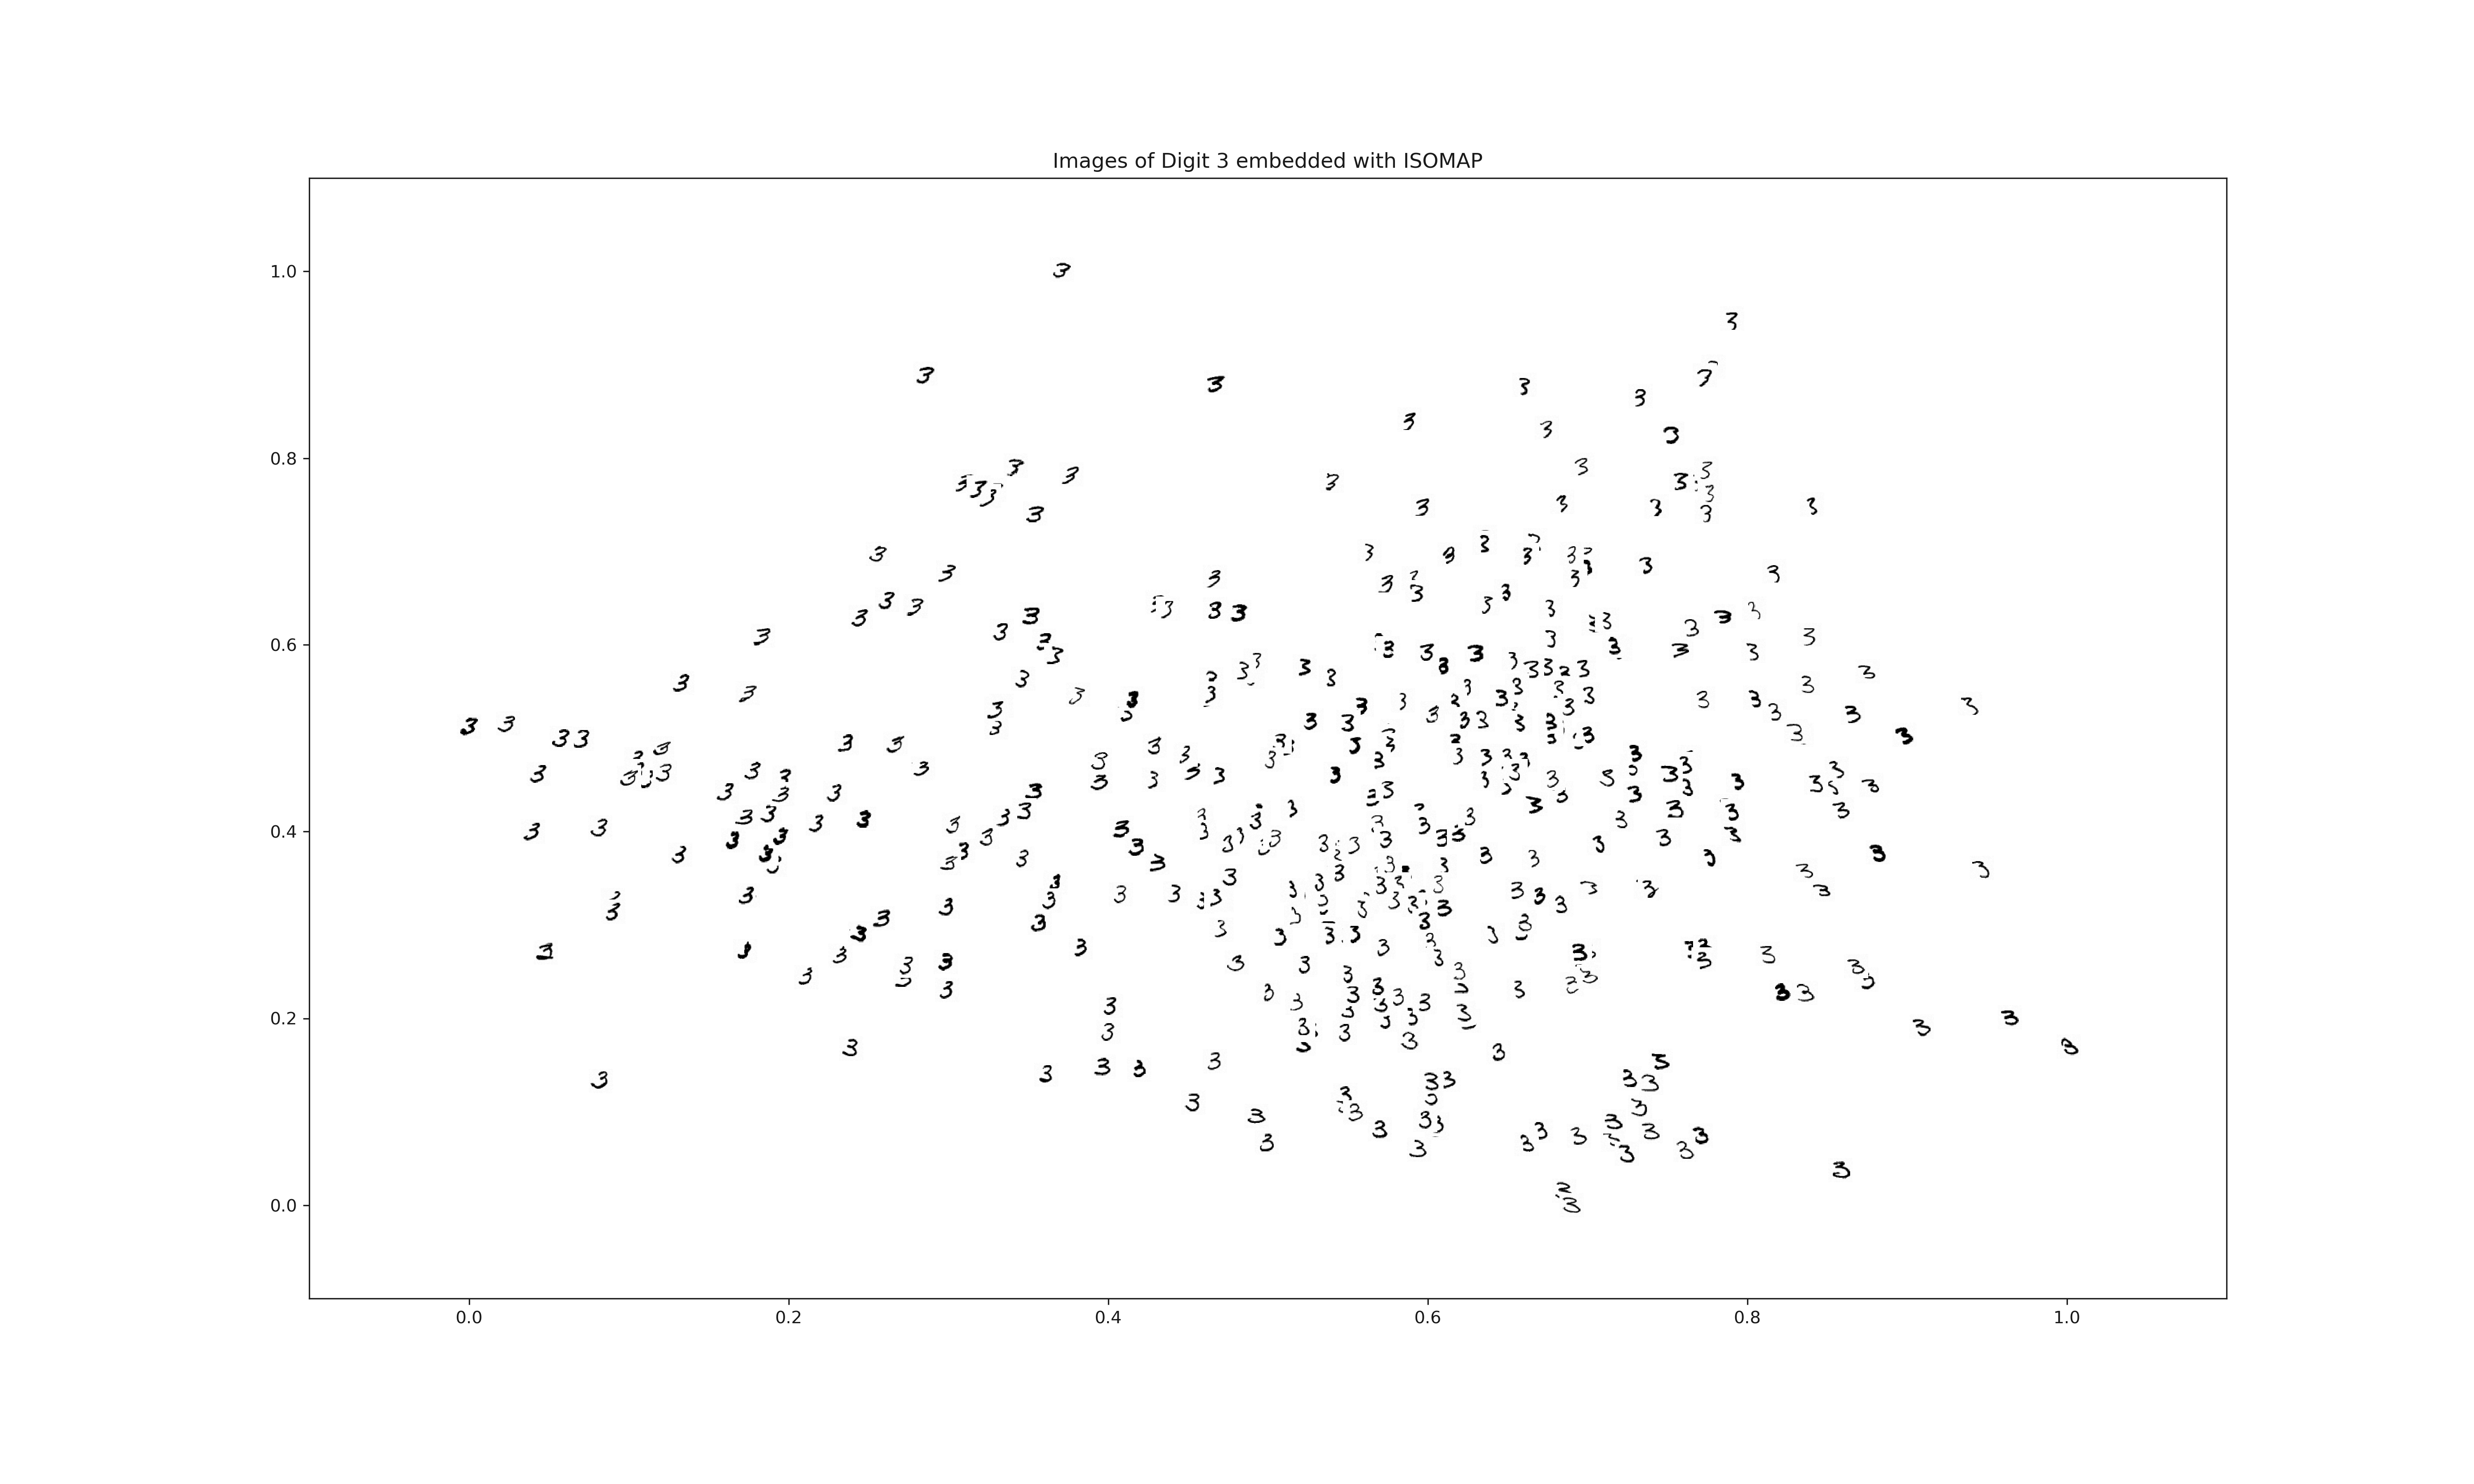
\includegraphics[width=\textwidth]{assignment1/3-2-ISOMAPembedding.png}
% \caption{\label{fig:fig10}Images of digit "3" embedded with Isomap}
% \end{figure}

% \clearpage{}
% \subsection{Naive Bayes classifier}

% The Naive Bayes classifier was used with both the dimensionally reduced data from the LLE and ISOMAP transformations. A train test split of 70/30 was used to separate the data and benchmark the performance of the classifier. This was repeated 30 times randomly sampling different partitions of the data set. A random seed was set at the beginning of the loop to ensure repeatable results when executing the notebook. PCA and LDA dimensionality reduced sets were also bench marked using the same training test splits. The results can be seen in Table~\ref{table:1}. the LDA trained Naive Bayes model performed the best with a very good predictive accuracy of 99\%. This could be because LDA is performed using the labelled data to help create boundaries between the digits in the data set. ISOMAP and PCA performed similarly while LLE performed a fair amount better than the other two. We decided to train and score the models 30 times and average the results. We feel this is a representative sample because the standard deviation of the runs is very small at around 1\% for each method. The central limit theorem states that the mean obtained from the sample will approximately equal true mean of the population. A rule of thumb to apply the theory is to have a sample size greater than 30.


% % \begin{table}
% % \caption{Performance Results of Naive Bayes Classifier.}\label{tab1}
% % \begin{tabular}{|l|l|l|}
% % \hline
% % Heading level &  Example & Font size and style\\
% % \hline
% % Title (centered) &  {\Large\bfseries Lecture Notes} & 14 point, bold\\
% % 1st-level heading &  {\large\bfseries 1 Introduction} & 12 point, bold\\
% % 2nd-level heading & {\bfseries 2.1 Printing Area} & 10 point, bold\\
% % 3rd-level heading & {\bfseries Run-in Heading in Bold.} Text follows & 10 point, bold\\
% % 4th-level heading & {\itshape Lowest Level Heading.} Text follows & 10 point, italic\\
% % \hline
% % \end{tabular}
% % \end{table}

% \begin{table}[h!]
% \caption{Performance Results of Naive Bayes Classifier}
% \label{table:1}
% \centering
%  \begin{tabular}{||c c c||} 
%  \hline
%  Mapping & Accuracy & Standard deviation \\ [0.5ex] 
%  \hline\hline
%  ISOMAP & 0.804 & 0.011 \\ 
%  \hline
%  LLE & 0.867 & 0.012 \\
%  \hline
%  PCA & 0.788 & 0.01 \\
%  \hline
%  LDA & 0.994 & 0.003 \\ [1ex] 
%  \hline
% \end{tabular}
% \end{table}
% % 4 dimsenional ISOMAP predicts with 0.804 accuracy and 0.011 standard deviation
% % 4 dimsenional LLE predicts with 0.867 accuracy and 0.012 standard deviation
% % 4 dimsenional PCA predicts with 0.788 accuracy and 0.010 standard deviation
% % 4 dimsenional LDA predicts with 0.994 accuracy and 0.003 standard deviation